\documentclass[a4paper, 12pt, french]{article}
\usepackage[utf8]{inputenc}
\usepackage[T1]{fontenc}
\usepackage{babel}[french]
\usepackage{amsmath,amssymb}
\usepackage{graphicx}
\usepackage{subfig}
\usepackage[colorinlistoftodos]{todonotes}
\usepackage{multicol}
\usepackage{indentfirst}
\usepackage{verbatim}
\usepackage{textcomp}
\usepackage{gensymb}
\usepackage{hyperref}
\usepackage{algorithm}
\usepackage[noend]{algpseudocode}
\usepackage{algorithmicx}
\usepackage{listingsutf8}
\usepackage{fancyhdr}
\definecolor{lightgray}{rgb}{.93,.94,.95}

\usepackage[T1]{fontenc}
\usepackage[scaled=0.85]{beramono}
\usepackage{listings}
\lstset{frameshape={RYR}{Y}{Y}{RYR},language=SQL,morekeywords={PREFIX,java,rdf,rdfs,url} extendedchars,
backgroundcolor=\color{lightgray},
showstringspaces=false, literate=%
		{'}{{'}}1 %permet l'écriture d'une apostrophe
		{é}{{\'e}}1
		{à}{{\`a}}1
		{ç}{{\c{c}}}1
		{œ}{{\oe}}1
		{ù}{{\`u}}1
		{É}{{\'E}}1
		{È}{{\`E}}1
		{À}{{\`A}}1
		{Ç}{{\c{C}}}1
		{Œ}{{\OE}}1
		{Ê}{{\^E}}1
		{ê}{{\^e}}1
		{î}{{\^i}}1
		{ô}{{\^o}}1
		{è}{{\`e}}1}


\usepackage{lineno}
\usepackage{float}
\usepackage{color}
\usepackage{lineno,hyperref}
\usepackage{ulem}
\setlength{\parindent}{0mm}
\usepackage{relsize}

\usepackage{lipsum}% http://ctan.org/pkg/lipsum
\usepackage{xcolor}% http://ctan.org/pkg/xcolor
\usepackage{xparse}% http://ctan.org/pkg/xparse
\NewDocumentCommand{\myrule}{O{1pt} O{2pt} O{black}}{%
  \par\nobreak % don't break a page here
  \kern\the\prevdepth % don't take into account the depth of the preceding line
  \kern#2 % space before the rule
  {\color{#3}\hrule height #1 width\hsize} % the rule
  \kern#2 % space after the rule
  \nointerlineskip % no additional space after the rule
}
\usepackage[section]{placeins}

\usepackage{pgfplots}
\pgfplotsset{compat=1.18}
\usepackage{booktabs}
\usepackage{tabularx}
\usepackage{seqsplit}
\usepackage{colortbl}%
   \newcommand{\myrowcolour}{\rowcolor[gray]{0.925}}
   
%\usepackage[obeyspaces]{url}
\usepackage{etoolbox}
%\usepackage[colorlinks,citecolor=black,urlcolor=blue,bookmarks=false,hypertexnames=true]{hyperref} 


\usepackage{geometry}
\geometry{
	paper=a4paper, % Change to letterpaper for US letter
	inner=3cm, % Inner margin
	outer=3cm, % Outer margin
	bindingoffset=.5cm, % Binding offset
	top=2cm, % Top margin
	bottom=2cm, % Bottom margin
	%showframe, % Uncomment to show how the type block is set on the page
}

\setlength{\headheight}{17.2pt}
\pagestyle{fancy}
\lhead{INF8085 Cybersécurité}
\rhead{Hiver 2026}
\renewcommand\footrulewidth{1pt}
\usepackage{listings}
\usepackage{color}
%*******************************************************************************%
\newcommand{\grando}[1]{O\mathopen{}\left(#1\right)}
%************************************START**************************************%
%*******************************************************************************%
\begin{document}

%*****************************TITLE PAGE*******************************%
\begin{titlepage}
\begin{center}
\textbf{\LARGE \'Ecole Polytechnique de Montr\'eal}\\[0.5cm] 
\textbf{\large D\'epartement de g\'enie informatique et g\'enie logiciel}\\[0.2cm]
\vspace{20pt}
\begin{figure}
 	\begin{center}	\includegraphics[width=90mm,scale=1.0]{images/poly.png}
	\end{center}
\end{figure}

\par
\vspace{20pt}
\vspace{15pt}
\myrule[1pt][7pt]
\textbf{\LARGE  Rapport du TP1}\\
\vspace{7pt}
\textbf{Cybersécurité}\\
\vspace{6pt}
\textbf{\large Travail pratique 1}\\
\myrule[1pt][7pt]

\vspace{25pt}

{\bfseries Fares Laadjel,} 2297799\\*[8pt]
{\bfseries Julien Cyr,} 2278776\\*[8pt]


\vspace{45pt}

\end{center}

\par
\vfill

\end{titlepage}





%********************************%
%***********  TOC  ************%
%********************************%
\tableofcontents
\newpage

%*******************************************************************************%
\section{Travail demandé}
%*******************************************************************************%

%-------------------------------------------------------------------------------%
\subsection{Entropie et sources d'information (10 points)}
%-------------------------------------------------------------------------------%
\begin{enumerate}
\item Supposez un alphabet de 50 symboles et une source qui produit un fichier de 500 caractères où chaque symbole a une probabilité égale de survenir. Quelle sera l'entropie moyenne théorique par lettre? Fournir le détail du calcul. /3

\vspace{0.8em}
\noindent\textbf{Étape 1 : probabilité de chaque symbole.}
\[
p_i = \frac{1}{50}, \quad \text{pour } i = 1, 2, \ldots, 50.
\]
\medskip
\noindent\textbf{Étape 2 : entropie de Shannon.}
\[
H(X) = -\sum_{i=1}^{50} p_i \log_2(p_i).
\]
\begin{center}
Puisque les $p_i$ sont identiques :
\end{center}
\[
H(X) = -50 \times \frac{1}{50} \times \log_2\left(\frac{1}{50}\right) = \log_2(50).
\]
\medskip
\noindent\textbf{Étape 3 : calcul numérique.}
\[
\log_2(50) = \frac{\ln(50)}{\ln(2)} \approx \frac{3{,}9120}{0{,}6931} \approx 5{,}644.
\]
\medskip

\noindent\textit{L'entropie moyenne théorique par lettre est donc d'environ 5,64 bits. Cela signifie qu'en moyenne, il faut environ 5,64 bits pour coder un symbole de cet alphabet sans perte.}

\vspace{1.2em}
\item Peut-on dire que cette entropie est maximale? Pourquoi? /2

\vspace{0.6em}
\textit{Oui, l'entropie est maximale. En effet, pour un alphabet donné, l'entropie atteint sa valeur maximale lorsque tous les symboles possibles sont équiprobables. Dans ce cas, la source est totalement imprévisible, ce qui maximise l'information moyenne par symbole.}

\vspace{1.2em}
\item En considérant seulement le contenu du fichier en lui-même, serait-il possible de réduire la taille du fichier en utilisant un algorithme de compression standard? Expliquez en vous basant sur le principe du taux de compression. /3

\vspace{0.6em}
\textit{Non, il ne serait pas possible de réduire la taille du fichier à l'aide d'un algorithme de compression standard, en considérant uniquement son contenu.}

\medskip\noindent
\textit{En effet, la source produit des symboles équiprobables, ce qui implique une entropie maximale égale à $\log_2(N)$ bits par symbole. Dans ce cas, le nombre moyen de bits nécessaires pour représenter chaque symbole correspond déjà à la limite théorique minimale. Il n'existe donc aucune redondance statistique exploitable par un algorithme de compression sans perte.}

\medskip\noindent
\textit{Selon le principe du taux de compression, lorsque l'entropie par symbole est égale au nombre de bits requis dans le pire cas, le taux de compression est égal à 1, ce qui signifie qu'aucun gain de compression n'est possible.}

\vspace{1.2em}
\item Concluez, en faisant un lien avec vos précédentes réponses, ce qui permet de compresser des images, ou encore du texte suivi, sans nécessairement faire référence à un algorithme de compression spécifique. /2

\vspace{0.6em}
\textit{Les images et les textes suivis sont compressibles parce qu'ils ne sont pas constitués de symboles indépendants et équiprobables. Ils présentent des régularités et des dépendances, par exemple certaines valeurs de pixels ou certaines lettres et suites de lettres apparaissent beaucoup plus souvent que d'autres. Cette redondance réduit l'entropie moyenne par symbole par rapport au cas d'entropie maximale. Comme l'information n'est pas répartie uniformément, il est alors possible de représenter le contenu avec moins de bits sans perte, contrairement à une source aléatoire uniforme.}

\end{enumerate}

%-------------------------------------------------------------------------------%
\subsection{La librairie de Babel (10 points)}
%-------------------------------------------------------------------------------%
\begin{enumerate}
\item Avec le premier matricule, récupérez le texte à matricule, wall 1, shelf 1, volume 1, page 1. Puis, calculez l'entropie par octet de ce texte (h-ascii). /2

\vspace{0.6em}
\begin{center}
\includegraphics[width=0.85\textwidth]{images/1.2.1.png}
\end{center}

\item Ajoutez, à la suite du texte initial, le texte trouvé avec le deuxième matricule. Puis, calculez l'entropie par octet de ce texte (h-ascii). /2

\vspace{0.6em}
\begin{center}
\includegraphics[width=0.85\textwidth]{images/1.2.2.png}
\end{center}

\item Discutez de la variation d'entropie que vous observez. /3

\vspace{0.6em}
\textit{On observe que l'entropie par octet varie très peu lorsqu'on ajoute le second texte au premier. Cette faible variation s'explique par le fait que l'entropie dépend uniquement de la distribution des symboles présents dans le texte. En concaténant deux textes issus de la librairie de Babel, on modifie légèrement les fréquences des caractères, mais sans changer leur répartition globale de manière significative.}

\medskip\noindent
\textit{Comme les deux textes proviennent de la même source et sont générés selon le même principe, leurs distributions de caractères sont similaires. L'ajout du second texte n'introduit donc pas de nouvelle structure ou régularité, ce qui explique que l'entropie reste pratiquement inchangée, avec seulement une légère variation due à l'ajustement des fréquences observées.}

\item Discutez de l'entropie de la librairie de Babel. /3

\vspace{0.6em}
\textit{L'entropie de la librairie de Babel, mesurée avec h-ascii, est d'environ 4,9 bits/octet pour les extraits considérés et demeure très proche lorsqu'on concatène plusieurs pages. Cela indique que, pour cette source, la distribution des octets observés est relativement stable d'un extrait à l'autre.}

\medskip\noindent
\textit{Pour interpréter cette valeur, il faut tenir compte du fait que la librairie de Babel utilise un alphabet restreint : elle ne mobilise pas forcément tous les 256 octets possibles. Le plafond pertinent est donc $\log_2(|\text{alphabet}|)$, et non pas 8 bits/octet. Dans ce cadre, une entropie vers 4{,}9 bits/octet peut être proche du maximum pour cet alphabet restreint si la distribution y est relativement uniforme.}

\medskip\noindent
\textit{En résumé, les pages de la librairie de Babel se comportent comme des sorties d'une même source dont les statistiques de symboles (octets) sont stables, ce qui se reflète par une entropie par octet voisine entre différents extraits.}

\end{enumerate}

%-------------------------------------------------------------------------------%
\subsection{Histogrammes (5 points)}
%-------------------------------------------------------------------------------%
\begin{enumerate}
\item Utilisez la librairie de Babel pour trouver un texte avec votre prénom et des mots en anglais aléatoires. Donnez ce texte (lettres majuscules et espaces uniquement, pas de chiffres). Modifiez le texte trouvé si nécessaire.

\vspace{0.6em}
\textit{CARPENTERS REDISTRIBUTE DISQUISITIONS ORNAMENTED UNHYSTERICAL CLAIRCOLLES UNHALLOW OLEORESINS FARES BESTSELLERDOM UNGENTLEMANLIKE FERMENTATIVE RACILY ANTICOAGULANTS REREWARDS SLINKER}

\item Utilisez CyberChef pour chiffrer ce texte avec ROT13. Assurez-vous que le résultat ne contienne que des lettres majuscules et des espaces.

\vspace{0.6em}
\textit{PNECRAGREF ERQVFGEVOHGR QVFDHVFVGVBAF BEANZRAGRQ HAULFGREVPNY PYNVEPBYYRF HAUNYYBJ BYRBERFVAF SNERF ORFGFRYYREQBZ HATRAGYRZNAYVXR SREZRAGNGVIR ENPVYL NAGVPBNTHYNAGF ERERJNEQF FYVAXRE}

\item Utilisez h-lettre sur la version avec ROT13 et sur la version sans ROT13, puis faites deux histogrammes avec un tableur. /1

\vspace{0.6em}
\begin{center}
\includegraphics[width=0.85\textwidth]{images/1.3.3.png}
\end{center}

\medskip
\noindent\textbf{Sortie h-lettre (données utilisées).}
\begin{lstlisting}[breaklines=true, basicstyle=\ttfamily\small, breakatwhitespace=false]
./h-lettre < Cyberchef-ROT13.txt
(space)=15 A=14 B=8 C=1 D=1 E=16 F=15 G=12 H=6 I=1 J=2 K=0 L=2
M=0 N=13 O=2 P=6 Q=5 R=23 S=2 T=2 U=2 V=14 W=0 X=2 Y=14 Z=4
Nombre total : 182  Entropie : 4.074212

./h-lettre < Cyberchef-original.txt
(space)=15 A=13 B=2 C=6 D=5 E=23 F=2 G=2 H=2 I=14 J=0 K=2 L=14
M=4 N=14 O=8 P=1 Q=1 R=16 S=15 T=12 U=6 V=1 W=2 X=0 Y=2 Z=0
Nombre total : 182  Entropie : 4.074212
\end{lstlisting}

\medskip
\noindent\textbf{Histogrammes (fréquences par caractère).}

\begin{center}
\begin{tikzpicture}
\begin{axis}[
  ybar, width=0.95\textwidth, height=7cm,
  ymin=0, ymax=25,
  symbolic x coords={Sp,A,B,C,D,E,F,G,H,I,J,K,L,M,N,O,P,Q,R,S,T,U,V,W,X,Y,Z},
  xtick=data, x tick label style={font=\small, rotate=45, anchor=east},
  ylabel={Occurrences},
  title={Version ROT13},
  bar width=8pt,
]
\addplot coordinates {
  (Sp,15)(A,14)(B,8)(C,1)(D,1)(E,16)(F,15)(G,12)(H,6)(I,1)(J,2)(K,0)(L,2)
  (M,0)(N,13)(O,2)(P,6)(Q,5)(R,23)(S,2)(T,2)(U,2)(V,14)(W,0)(X,2)(Y,14)(Z,4)
};
\end{axis}
\end{tikzpicture}

\vspace{1em}
\begin{tikzpicture}
\begin{axis}[
  ybar, width=0.95\textwidth, height=7cm,
  ymin=0, ymax=25,
  symbolic x coords={Sp,A,B,C,D,E,F,G,H,I,J,K,L,M,N,O,P,Q,R,S,T,U,V,W,X,Y,Z},
  xtick=data, x tick label style={font=\small, rotate=45, anchor=east},
  ylabel={Occurrences},
  title={Version originale},
  bar width=8pt,
]
\addplot coordinates {
  (Sp,15)(A,13)(B,2)(C,6)(D,5)(E,23)(F,2)(G,2)(H,2)(I,14)(J,0)(K,2)(L,14)
  (M,4)(N,14)(O,8)(P,1)(Q,1)(R,16)(S,15)(T,12)(U,6)(V,1)(W,2)(X,0)(Y,2)(Z,0)
};
\end{axis}
\end{tikzpicture}
\end{center}
\noindent{\footnotesize (Sp = espace; entropie dans les deux cas : 4{,}074212.)}

\item Utilisez le programme lettre pour générer une séquence de 3200 caractères, puis encodez cette séquence avec ROT13.

\vspace{0.6em}
\begin{center}
\textit{Voir le numéro ci-dessous.}
\end{center}

\item Utilisez h-lettre sur la version avec ROT13 et sur la version sans ROT13, puis faites deux histogrammes avec un tableur. /1

\vspace{0.6em}
\begin{center}
\includegraphics[width=0.85\textwidth]{images/1.3.5.png}
\end{center}

\medskip
\noindent\textbf{Sortie h-lettre (données utilisées).}
\begin{lstlisting}[breaklines=true, basicstyle=\ttfamily\small, breakatwhitespace=false]
./h-lettre < Lettre-original.txt
(space)=371 A=231 B=42 C=85 D=117 E=334 F=64 G=72 H=171 I=203 J=11 K=29 L=115
M=69 N=203 O=215 P=55 Q=7 R=148 S=173 T=238 U=81 V=32 W=57 X=2 Y=73 Z=2
Nombre total : 3200  Entropie : 4.253363

./h-lettre < Lettre-ROT13.txt
(space)=371 A=203 B=215 C=55 D=7 E=148 F=173 G=238 H=81 I=32 J=57 K=2 L=73
M=2 N=231 O=42 P=85 Q=117 R=334 S=64 T=72 U=171 V=203 W=11 X=29 Y=115 Z=69
Nombre total : 3200  Entropie : 4.253363
\end{lstlisting}

\medskip
\noindent\textbf{Histogrammes (fréquences par caractère).}

\begin{center}
\begin{tikzpicture}
\begin{axis}[
  ybar, width=0.95\textwidth, height=7cm,
  ymin=0, ymax=380,
  symbolic x coords={Sp,A,B,C,D,E,F,G,H,I,J,K,L,M,N,O,P,Q,R,S,T,U,V,W,X,Y,Z},
  xtick=data, x tick label style={font=\small, rotate=45, anchor=east},
  ylabel={Occurrences},
  title={Lettre originale (3200 car.)},
  bar width=8pt,
]
\addplot coordinates {
  (Sp,371)(A,231)(B,42)(C,85)(D,117)(E,334)(F,64)(G,72)(H,171)(I,203)(J,11)(K,29)(L,115)
  (M,69)(N,203)(O,215)(P,55)(Q,7)(R,148)(S,173)(T,238)(U,81)(V,32)(W,57)(X,2)(Y,73)(Z,2)
};
\end{axis}
\end{tikzpicture}

\vspace{1em}
\begin{tikzpicture}
\begin{axis}[
  ybar, width=0.95\textwidth, height=7cm,
  ymin=0, ymax=380,
  symbolic x coords={Sp,A,B,C,D,E,F,G,H,I,J,K,L,M,N,O,P,Q,R,S,T,U,V,W,X,Y,Z},
  xtick=data, x tick label style={font=\small, rotate=45, anchor=east},
  ylabel={Occurrences},
  title={Lettre ROT13 (3200 car.)},
  bar width=8pt,
]
\addplot coordinates {
  (Sp,371)(A,203)(B,215)(C,55)(D,7)(E,148)(F,173)(G,238)(H,81)(I,32)(J,57)(K,2)(L,73)
  (M,2)(N,231)(O,42)(P,85)(Q,117)(R,334)(S,64)(T,72)(U,171)(V,203)(W,11)(X,29)(Y,115)(Z,69)
};
\end{axis}
\end{tikzpicture}
\end{center}
\noindent{\footnotesize (Sp = espace; entropie dans les deux cas : 4{,}253363.)}

\item Que remarquez-vous en comparant ces quatre histogrammes? Comment seraient les histogrammes des sources lettre et texte si les fréquences étaient comptabilisées sur deux lettres à la fois? Comment devrait être par exemple les fréquences du (ee) et du (th) dans le cas de texte et de lettre? /1,5

\vspace{0.6em}
\textit{En comparant les quatre histogrammes, on observe que le chiffrement ROT13 ne modifie pas les fréquences globales des caractères, mais les associe à d'autres lettres. Les histogrammes avant et après ROT13 ne sont donc pas identiques lettre par lettre : les barres de forte occurrence sont simplement déplacées le long de l'axe des lettres. Ce comportement est caractéristique d'un chiffrement par substitution.}

\medskip\noindent
\textit{On remarque également une différence entre les histogrammes issus de la source lettre et ceux issus du texte de la librairie de Babel. La source lettre, générée selon les fréquences de l'anglais, présente une structure plus marquée avec certaines lettres et l'espace beaucoup plus fréquents. À l'inverse, le texte Babel, surtout lorsqu'il est court, produit des histogrammes plus irréguliers, ce qui reflète une absence de structure linguistique stable.}

\medskip\noindent
\textit{Si les fréquences étaient comptabilisées sur deux lettres à la fois (digrammes), ces différences seraient encore plus visibles. Dans le cas de la source texte (anglais), certains digrammes courants comme (th) ou (ee) auraient des fréquences nettement plus élevées que les autres. En revanche, pour la source lettre, où les lettres sont générées indépendamment les unes des autres, les digrammes seraient beaucoup plus uniformément répartis et des digrammes comme (th) ou (ee) ne seraient pas particulièrement favorisés.}

\item Est-ce que comptabiliser les fréquences sur 2 lettres faciliterait le déchiffrement du message dans le cas du texte pris sur Babel? Qu'en est-il pour celui généré avec lettre? /1,5

\vspace{0.6em}
\textit{Dans le cas du texte pris sur la librairie de Babel, comme l'extrait analysé contient de nombreux mots anglais valides, il présente des régularités locales propres à la langue. Le comptage des fréquences sur deux lettres (digrammes) mettrait alors en évidence des paires courantes de l'anglais, telles que th, er, re ou ll, ce qui fournirait des indices supplémentaires utiles pour le déchiffrement d'un chiffrement par substitution.}

\medskip\noindent
\textit{En revanche, pour le texte généré avec la source lettre, les lettres sont produites indépendamment les unes des autres selon une distribution donnée. Il n'existe donc pas de dépendance entre lettres successives, et le comptage des fréquences sur deux lettres n'apporte pas d'information supplémentaire par rapport à l'analyse lettre par lettre. Les digrammes comme th ou ee n'y sont pas favorisés et ne facilitent pas le déchiffrement.}

\end{enumerate}

%-------------------------------------------------------------------------------%
\subsection{Déchiffrement simple (15 points)}
%-------------------------------------------------------------------------------%
\begin{enumerate}
\item Donnez une capture d'écran de votre utilisation de l'utilitaire frequency. /1

\vspace{0.6em}
\begin{center}
\includegraphics[width=0.85\textwidth]{images/dechiffrement.png}
\end{center}

\item Fournir le texte déchiffré, ainsi que votre démarche clairement expliquée. /14

\vspace{0.6em}
\noindent\textbf{Texte déchiffré :}\\[0.4em]
\textit{ urotherwas saying  it was merely a few words of encouragement the sort of words thatare uttered in the din of battle not distinguishable individually but restoringconfidence by the fact of being spok }

\medskip
\noindent\textbf{Démarche.}
\textit{Le déchiffrement a été effectué par analyse fréquentielle suivie d'une déduction progressive appliquée séquentiellement.}

\medskip\noindent
\textit{Dans un premier temps, l'utilitaire frequency a été utilisé pour mesurer les fréquences des caractères du message chiffré. Les résultats ont été triés avec sort -k3 -nr afin d'identifier rapidement les symboles dominants. La distribution observée étant compatible avec l'anglais, le symbole le plus fréquent a été associé à l'espace, conformément à l'indication fournie dans l'énoncé. Cette étape a servi de base pour construire une table de substitution initiale.}

\medskip\noindent
\textit{L'analyse des digrammes et trigrammes a ensuite permis d'identifier des motifs probables. Le trigramme XJS a été reconnu comme correspondant au mot très fréquent the, ce qui a permis de déduire X → t et J → h. Le digramme IW a ensuite été identifié comme in, menant à I → i et W → n. Ces substitutions ont immédiatement rendu plusieurs fragments de texte partiellement lisibles, confirmant la validité des hypothèses.}

\medskip\noindent
\textit{La progression s'est poursuivie par reconnaissance de mots lisibles par contexte. Par exemple, la séquence UeinO correspondait clairement à being, ce qui a permis d'associer U → b et O → g. Le digramme bD a été identifié comme by, donnant D → y, et LT comme of. La lettre C a été confirmée par apparition dans des mots cohérents.}

\medskip\noindent
\textit{À ce stade, plusieurs mots entiers devenaient reconnaissables : encouragement, few, words, battle, individually. Ces reconnaissances ont permis de valider les substitutions existantes et d'en proposer de nouvelles, notamment G → a, afin de préserver la cohérence grammaticale globale.}

\medskip\noindent
\textit{Les lettres restantes correspondaient à des symboles de faible fréquence, cohérents avec des lettres rares en anglais. La résolution finale s'est appuyée sur la structure grammaticale de la phrase et sur la plausibilité linguistique globale, confirmant la cohérence du message reconstruit.}

\medskip\noindent
\textit{Le déchiffrement a donc été réalisé par une combinaison d'analyse statistique, d'identification de motifs fréquents, d'application progressive des substitutions et de validation contextuelle jusqu'à obtention d'un texte cohérent.}
\end{enumerate}

%-------------------------------------------------------------------------------%
\subsection{Masque jetable (20 points)}
%-------------------------------------------------------------------------------%
\begin{enumerate}
\item Créez un programme qui génère en binaire un masque jetable (probabilité égale 0/1). Donnez le code, expliquez le fonctionnement. Utilisez le module random de base et une alternative plus sécuritaire; expliquez en quoi cette alternative est plus sécuritaire. /12

\vspace{0.6em}
\textit{Le programme ci-dessous génère un masque jetable sous forme binaire, stocké dans un fichier \texttt{key.txt}. Le masque est une suite d'octets, de longueur \texttt{size} octets, afin de correspondre à la taille du message à chiffrer en octets, condition requise pour un masque jetable (OTP).}

\medskip\noindent
\textit{Chaque octet est tiré uniformément parmi 0..255. Cette uniformité implique que, pour chaque position de bit (parmi les 8 bits d'un octet), la probabilité d'obtenir 0 ou 1 est égale à 1/2, car sur les 256 valeurs possibles, 128 ont ce bit à 0 et 128 l'ont à 1.}

\medskip\noindent
\textit{La version non sécuritaire utilise le module \texttt{random} (tirages pseudo-aléatoires déterministes), tandis que la version sécuritaire utilise \texttt{secrets}, conçu pour la cryptographie et s'appuyant sur une source d'aléa du système d'exploitation.}

\medskip
\begin{lstlisting}[language=Python, basicstyle=\small\ttfamily, breaklines=true, frame=single]
from random import randint
import secrets
import sys

def notSecureKey(size: int) -> None:
    # Génère size octets pseudo-aléatoires (non cryptographiques)
    with open("key.txt", "wb") as key_file:
        for _ in range(size):
            k = randint(0, 255)
            key_file.write(bytes([k]))

def secureKey(size: int) -> None:
    # Génère size octets avec une source adaptée à la cryptographie
    with open("key.txt", "wb") as key_file:
        key_file.write(secrets.token_bytes(size))

secureKey(100) if sys.argv[1] == "secure" else notSecureKey(100)
\end{lstlisting}

\medskip\noindent
\textit{\textbf{Sécurité des deux méthodes.} Le module \texttt{random} produit une suite pseudo-aléatoire déterministe basée sur un état interne. Si cet état est récupéré ou deviné, la suite peut devenir prédictible, ce qui est incompatible avec les exigences de sécurité d'un OTP. Le module \texttt{secrets} est conçu pour générer des valeurs non prédictibles pour un attaquant, en utilisant une source d'aléa cryptographiquement robuste fournie par le système d'exploitation~\cite{secrets}.}

\item Utilisez votre programme pour générer des clés pour les 100 premiers caractères du texte de 4.3.1 (sans espaces). D'abord avec random de base, puis avec l'alternative sécuritaire.

\vspace{0.6em}
\textit{Le fichier \texttt{smallText.txt} est produit par le programme, en retirant les espaces du texte puis en conservant les 100 premiers caractères. Ensuite, on génère une clé de 100 octets et on l'écrit dans \texttt{key.txt}.}

\medskip\noindent
\textbf{Commandes utilisées :}
\begin{verbatim}
python3 otp.py random
python3 otp.py secure
\end{verbatim}

\begin{center}
\includegraphics[width=0.85\textwidth]{images/1.5.2.png}
\end{center}

\item Utilisez l'utilitaire masque pour appliquer vos clés sur le texte. Calculez l'entropie par bit (h-bit) et par octet (h-ascii) avant et après l'application de chaque masque. /3

\vspace{0.6em}
\begin{center}
\includegraphics[width=0.85\textwidth]{images/1.5.3.png}
\end{center}

\item Discutez des résultats. Dites à quoi vous vous attendiez, si les résultats sont conformes ou non, et pourquoi. /5

\vspace{0.6em}
\textit{Avant l'application du masque jetable, l'entropie est limitée par la structure du texte : l'alphabet est restreint (lettres majuscules) et les fréquences ne sont pas uniformes, ce qui explique une entropie par octet d'environ 3{,}87 et une entropie par bit d'environ 0{,}97.}

\medskip\noindent
\textit{Après application du masque jetable, l'entropie par bit devient très proche de 1 dans les deux cas, ce qui est conforme à l'attendu : le XOR avec une clé aléatoire de même longueur rend les bits de sortie proches d'une distribution équilibrée 0/1.}

\medskip\noindent
\textit{L'entropie par octet du texte chiffré se situe autour de 6{,}2--6{,}3 bits/octet pour un fichier de 100 octets. Cette valeur est cohérente avec la taille de l'échantillon : avec seulement 100 octets observés, l'entropie empirique par octet ne peut pas atteindre 8, et elle est bornée par $\log_2(100) \approx 6{,}64$ bits/octet. Avec davantage d'octets chiffrés, l'estimation se rapprocherait de 8 bits/octet.}

\medskip\noindent
\textit{Les résultats random et secure sont proches du point de vue de l'entropie mesurée sur un petit échantillon. La différence principale entre les deux méthodes est la prédictibilité : random n'est pas conçu pour des usages cryptographiques, alors que secrets vise l'imprévisibilité face à un attaquant, ce qui est requis pour la sécurité effective d'un OTP.}

\end{enumerate}

%-------------------------------------------------------------------------------%
\subsection{Communication à clé publique, HTTPS et SSL (5 points)}
%-------------------------------------------------------------------------------%
\begin{enumerate}
\item Expliquez la différence entre HTTP et HTTPS dans vos mots. /0,5

\vspace{0.6em}
\textit{HTTP et HTTPS sont deux protocoles utilisés pour la communication entre un navigateur web et un serveur. La différence principale entre les deux réside dans la sécurité des échanges.}

\medskip\noindent
\textit{HTTP transmet les données en clair sur le réseau. Cela signifie que les informations échangées, comme les identifiants, mots de passe ou données personnelles, peuvent être interceptées et lues par un attaquant qui aurait accès au trafic réseau.}

\medskip\noindent
\textit{HTTPS est la version sécurisée de HTTP. Il utilise un chiffrement basé sur TLS afin de protéger les communications. Les données échangées sont chiffrées, ce qui empêche un tiers de les lire ou de les modifier. De plus, HTTPS permet au navigateur de vérifier l'identité du serveur grâce à un certificat numérique, ce qui réduit les risques d'usurpation de site~\cite{awshttps}.}

\item Expliquez pourquoi il est impossible de se connecter au dossier étudiant avec http et quelle solution sécuritaire pourrait être mise en place. /1

\vspace{0.6em}
\textit{Il est impossible de se connecter au dossier étudiant en utilisant le protocole HTTP, car ce service exige une communication sécurisée. Le dossier étudiant traite des informations sensibles, comme des données personnelles et académiques, qui ne doivent pas transiter en clair sur le réseau. Pour cette raison, le serveur refuse les connexions non chiffrées afin d'éviter les risques d'interception ou de modification des données par un attaquant.}

\medskip\noindent
\textit{Une solution sécuritaire consiste à forcer l'utilisation de HTTPS en redirigeant automatiquement toute requête HTTP vers la version HTTPS du site. Ainsi, même si un utilisateur consulte le lien en HTTP, la connexion est immédiatement établie de manière chiffrée, garantissant la confidentialité et l'intégrité des échanges.}

\item Quelle est l'utilité du header « Strict-Transport-Security »? /1

\vspace{0.6em}
\textit{Le header Strict-Transport-Security a pour rôle de forcer le navigateur à utiliser uniquement des connexions HTTPS pour un site donné pendant une durée déterminée. Lorsqu'un navigateur reçoit ce header, il mémorise que le site doit toujours être contacté via HTTPS, même si l'utilisateur tente d'y accéder en utilisant HTTP.}

\medskip\noindent
\textit{Ce mécanisme empêche les attaques de type « downgrade » ou « man-in-the-middle » où un attaquant tenterait de rediriger l'utilisateur vers une version non sécurisée du site. En imposant systématiquement le chiffrement des communications, Strict-Transport-Security renforce la sécurité globale des échanges entre le navigateur et le serveur~\cite{mdnhsts}.}

\item À quoi sert un certificat à clé publique? Comment votre navigateur vérifie-t-il l'identité du propriétaire du site? /0,5

\vspace{0.6em}
\textit{Un certificat à clé publique, aussi appelé certificat TLS (souvent désigné comme certificat SSL), sert à associer une clé publique à l'identité d'un site afin de permettre des communications sécurisées. Il est utilisé pour authentifier le serveur et établir une connexion chiffrée entre le navigateur et le site web.}

\medskip\noindent
\textit{Le navigateur vérifie l'identité du propriétaire du site lors de la négociation TLS en validant le certificat présenté par le serveur. Il s'assure que le certificat est signé par une autorité de certification de confiance, que le nom de domaine correspond au site visité et que le certificat est valide. Si ces vérifications sont satisfaites, le navigateur fait confiance à l'identité du site~\cite{cloudflaressl}.}

\item Utilisez openssl pour générer un certificat « Self-Signed ». Donnez dans un tableau les champs de votre certificat. /0,5

\vspace{0.6em}
\begin{center}
\includegraphics[width=0.85\textwidth]{images/1.6.5.png}
\end{center}

\medskip
\noindent Champs du certificat (sortie \texttt{openssl x509 -text})~\cite{baeldungopenssl} :

\footnotesize
\noindent\begin{tabularx}{\linewidth}{@{}>{\raggedright\arraybackslash}p{2.8cm}>{\raggedright\arraybackslash}X@{}}
\toprule
\textbf{Champ} & \textbf{Valeur} \\
\midrule
Version & 3 (0x2) \\
Serial Number & \seqsplit{15:07:de:79:5d:ef:14:97:92:36:65:02:24:6b:c0:24:e8:4a:dc:44} \\
Signature Algorithm & sha256WithRSAEncryption \\
Issuer & C=CA, ST=Quebec, L=Montreal, O=Kali, OU=Kali, CN=Kali, emailAddress=Kali \\
Not Before & Feb 2 00:57:56 2026 GMT \\
Not After & Feb 2 00:57:56 2027 GMT \\
Subject & C=CA, ST=Quebec, L=Montreal, O=Kali, OU=Kali, CN=Kali, emailAddress=Kali \\
Public Key Algorithm & rsaEncryption \\
Public-Key & 2048 bit \\
Exponent & 65537 (0x10001) \\
Subject Key Identifier & \seqsplit{FA:92:05:3A:AE:E3:AF:30:35:3F:F9:7F:64:EF:E4:E0:56:92:C5:EA} \\
\bottomrule
\end{tabularx}
\normalsize

\item Lancez un serveur python local qui utilise votre certificat (script fourni). Fournissez la clé et le certificat en format .pem.

\vspace{0.6em}
\begin{center}
\includegraphics[width=0.85\textwidth]{images/1.6.6.png}
\end{center}

\item Tentez d'accéder au serveur avec Firefox. Quel problème rencontrez-vous et comment le régler? Expliquez votre démarche. /1,5

\vspace{0.6em}
\begin{center}
\includegraphics[width=0.85\textwidth]{images/1.6.7.png}
\end{center}

\textit{Lors de l'accès au serveur HTTPS dans Firefox, le navigateur bloque la connexion et affiche un avertissement de sécurité indiquant que le certificat est invalide ou non approuvé. Le problème vient du fait que le certificat utilisé par le serveur est auto-signé. Il n'est donc pas signé par une autorité de certification reconnue par Firefox, ce qui empêche le navigateur de valider l'identité du serveur et d'établir une relation de confiance. Un code d'erreur du type MOZILLA\_PKIX\_ERROR\_SELF\_SIGNED\_CERT est affiché.}

\medskip\noindent
\textit{Pour régler ce problème dans le cadre du laboratoire, la démarche consiste à ajouter une exception de sécurité dans Firefox. En accédant à l'URL du serveur, on clique sur « Avancé » dans la page d'avertissement, puis on choisit l'option « Accepter le risque et poursuivre ». Firefox enregistre alors une exception locale pour ce site et permet l'accès au serveur via HTTPS. Cela confirme que le chiffrement TLS fonctionne, mais que le certificat n'était pas approuvé par défaut.}

\medskip\noindent
\textit{Une solution plus « propre » et permanente consisterait à utiliser un certificat signé par une autorité de certification de confiance, ou à créer une autorité de certification locale, l'ajouter comme autorité de confiance dans Firefox, puis signer le certificat du serveur avec cette autorité. Dans tous les cas, le problème initial observé est l'absence de chaîne de confiance reconnue pour un certificat auto-signé.}

\end{enumerate}

%-------------------------------------------------------------------------------%
\subsection{Codage (9 points)}
%-------------------------------------------------------------------------------%
\begin{enumerate}
\item Expliciter les alphabets $\sigma$, $\tau$ et $\tau'$ (sortie de la source, du codeur, du bloc de chiffrement). /3

\vspace{0.6em}
\textit{$\sigma$ est l'alphabet de sortie de la source, c'est-à-dire l'ensemble des symboles possibles d'un NIP. Il contient les dix chiffres et les vingt-six lettres majuscules : $\sigma = \{0,1,2,3,4,5,6,7,8,9,A,B,C,\ldots,Z\}$. Un NIP est une suite de 8 symboles appartenant à $\sigma$.}

\medskip\noindent
\textit{$\tau$ est l'alphabet de sortie du codeur, avant chiffrement. Chaque symbole de $\sigma$ est encodé en ASCII sur un octet, puis la suite de 8 octets est dupliquée. $\tau$ correspond donc à l'ensemble des valeurs ASCII des chiffres et des lettres majuscules : $\tau = \{0x30,\ldots,0x39, 0x41,\ldots,0x5A\}$. La sortie du codeur est une suite de 16 octets sur $\tau$.}

\medskip\noindent
\textit{$\tau'$ est l'alphabet du bloc de chiffrement AES-128. AES-128 manipule des blocs de taille fixe de 128 bits. $\tau'$ est donc l'ensemble de tous les blocs possibles de 128 bits, soit l'ensemble de toutes les suites possibles de 16 octets.}

\item Identifier les langages provenant de ces alphabets. /3

\vspace{0.6em}
\noindent\textbf{Langage sur $\sigma$.}

\textit{Le langage associé à l'alphabet $\sigma$ est l'ensemble de tous les NIP possibles. Il s'agit de toutes les suites de longueur 8 composées de symboles de $\sigma$.}

\textit{On peut l'écrire : $L(\sigma) = \sigma^8$.}

\medskip
\noindent\textbf{Langage sur $\tau$.}

\textit{Le langage associé à l'alphabet $\tau$ est l'ensemble des sorties possibles du codeur. Chaque mot est formé de 16 octets, correspondant à la répétition deux fois de l'encodage ASCII d'un NIP valide.}

\textit{Le langage est donc l'ensemble des mots de longueur 16 sur $\tau$ ayant la structure $X\|X$, où $X$ est une suite de 8 symboles de $\tau$ correspondant à un NIP valide.}

\medskip
\noindent\textbf{Langage sur $\tau'$.}

\textit{Le langage associé à l'alphabet $\tau'$ est l'ensemble des blocs pouvant être traités par AES-128. Il contient toutes les suites possibles de 128 bits, sans contrainte particulière de structure.}

\textit{On peut l'écrire : $L(\tau') = (\tau')^1$, c'est-à-dire l'ensemble de tous les blocs de 128 bits.}

\item Identifiez les attaques auxquelles le système est vulnérable. /3

\vspace{0.6em}
\textit{Premièrement, le système est vulnérable à une attaque par rejeu. Un attaquant peut intercepter un message chiffré correspondant à un changement de NIP et le réinjecter plus tard sur le réseau. Comme le message chiffré est toujours identique pour un même NIP et qu'aucune information temporelle ou aléatoire n'est incluse, la banque ne peut pas distinguer un message légitime d'un ancien message rejoué.}

\medskip\noindent
\textit{Deuxièmement, le système est vulnérable à une attaque par substitution. Un attaquant peut remplacer, sur le réseau, le message chiffré d'un client par un autre message chiffré valide qu'il a préalablement capturé. Étant donné que l'identité du client est supposée transmise de façon indépendante, le serveur peut associer à tort le NIP contenu dans le message substitué au mauvais compte.}

\medskip\noindent
\textit{Troisièmement, le système est vulnérable à une attaque par reconnaissance de motifs. Le codage étant déterministe, deux NIP identiques produisent exactement le même bloc clair, et donc le même bloc chiffré. Un attaquant observant le trafic peut détecter qu'un même NIP est réutilisé ou qu'un client revient à un ancien NIP, même sans connaître sa valeur.}

\medskip\noindent
\textit{Enfin, le système est vulnérable à une attaque par modification de message. Un attaquant peut altérer arbitrairement des bits du message chiffré. En l'absence de mécanisme d'authentification ou d'intégrité, le déchiffrement produira un NIP incohérent sans que la banque puisse détecter que le message a été modifié, ce qui peut mener à un déni de service ou à un état incohérent du système.}

\end{enumerate}

%-------------------------------------------------------------------------------%
\subsection{Changement de codage (5 points)}
%-------------------------------------------------------------------------------%
\begin{enumerate}
\item Pour chacun des trois codages (figures 1, 2, 3), dites quelles attaques du 4.7.3 ils permettent de bloquer. /3

\vspace{0.6em}
\noindent\textbf{Codage 1 (nouveau NIP + parité + nombre aléatoire).}

\textit{Ce codage permet de bloquer l'attaque par reconnaissance de motifs. L'ajout d'un nombre aléatoire fait que deux NIP identiques ne produisent plus le même bloc clair, et donc plus le même bloc chiffré.}

\textit{En revanche, il ne bloque pas l'attaque par rejeu, car un message chiffré ancien peut toujours être rejoué tel quel. Il ne bloque pas non plus l'attaque par substitution, puisqu'un message chiffré valide capturé peut être remplacé par un autre sur le réseau. Enfin, il ne protège pas contre l'attaque par modification de message, en l'absence de mécanisme d'intégrité.}

\medskip
\noindent\textbf{Codage 2 (nouveau NIP + parité + nombre aléatoire + horodatage).}

\textit{Ce codage permet de bloquer l'attaque par reconnaissance de motifs, grâce à la présence d'aléa. Il permet également de bloquer l'attaque par rejeu de messages anciens, puisque l'horodatage permet à la banque d'invalider les messages trop vieux.}

\textit{En revanche, il ne bloque pas complètement l'attaque par substitution, car un attaquant peut encore remplacer un message par un autre message récent dont l'horodatage est valide. Comme les autres, il ne protège pas contre l'attaque par modification de message, faute de mécanisme d'authentification ou d'intégrité.}

\medskip
\noindent\textbf{Codage 3 (nouveau NIP + ancien NIP + horodatage).}

\textit{Ce codage permet de bloquer l'attaque par rejeu, grâce à l'horodatage. Il permet aussi de bloquer l'attaque par substitution, car un message n'est accepté que si l'ancien NIP correspond à celui attendu par la banque pour le compte concerné, ce qu'un attaquant ne peut pas produire sans connaître cet ancien NIP.}

\textit{La reconnaissance de motifs est fortement limitée par la présence du timestamp, qui empêche la répétition exacte des blocs. En revanche, comme pour les autres codages, l'attaque par modification de message reste possible, puisqu'aucun mécanisme d'intégrité n'est ajouté.}

\item Selon vous, quel est le meilleur codage? Pourquoi? /2

\vspace{0.6em}
\textit{Le meilleur codage est le codage 3.}

\medskip\noindent
\textit{En effet, parmi les trois propositions, c'est le seul codage qui permet de bloquer l'attaque la plus critique dans ce scénario, à savoir l'attaque par substitution. En incluant l'ancien NIP dans le message, le changement de NIP est lié à l'état courant du compte, ce qui empêche un attaquant de réutiliser ou de substituer un message chiffré capturé pour un autre client sans connaître l'ancien NIP correspondant. De plus, la présence d'un horodatage permet de bloquer les attaques par rejeu de messages anciens.}

\medskip\noindent
\textit{Les codages 1 et 2 améliorent principalement la confidentialité face à l'observation du trafic en empêchant la reconnaissance de motifs, mais ils ne protègent pas contre la substitution de messages, qui est une attaque active plus dangereuse dans le modèle de menace considéré.}
\end{enumerate}

%-------------------------------------------------------------------------------%
\subsection{Chiffrement par bloc et modes d'opération (4 points)}
%-------------------------------------------------------------------------------%
\begin{enumerate}
\item Chiffrez le fichier mdp.jpg en mode ECB avec le script AES.py. Observez le fichier de sortie et commentez. /1

\vspace{0.6em}
\begin{center}
\includegraphics[width=0.85\textwidth]{images/mdp_bad.png}
\end{center}

\medskip\noindent
\textit{Le fichier mdp.jpg, contenant un mot de passe enregistré sous forme d'image, a été chiffré à l'aide du script AES.py en mode ECB. L'exécution de la commande \texttt{python3 AES.py -i mdp.jpg -m ECB} produit un fichier image chiffré (mdp\_enc.jpg).}

\medskip\noindent
\textit{À l'observation du fichier de sortie, on constate que l'image chiffrée conserve des structures visuelles reconnaissables de l'image originale, en particulier la forme et la position des lettres du mot « Password », bien que les couleurs soient altérées et semblent aléatoires. Cela s'explique par le fonctionnement du mode ECB : chaque bloc de 128 bits est chiffré indépendamment avec la même clé. Ainsi, deux blocs identiques en entrée produisent deux blocs identiques en sortie.}

\medskip\noindent
\textit{Dans une image, de nombreuses zones contiennent des pixels identiques ou très similaires. Le mode ECB préserve donc les motifs et les répétitions présentes dans les données, ce qui entraîne une fuite d'information visuelle malgré l'utilisation d'un algorithme de chiffrement considéré comme sécurisé (AES).}

\medskip\noindent
\textit{Cette expérience montre que, même si AES est cryptographiquement robuste, le mode ECB est inadapté pour chiffrer des données structurées comme des images, car il ne garantit pas la confidentialité des motifs et révèle des informations sur le contenu original.}

\item Chiffrez maintenant le fichier en mode CBC. Observez le fichier puis commentez. /1

\vspace{0.6em}
\begin{center}
\includegraphics[width=0.85\textwidth]{images/mdp_good.png}
\end{center}

\medskip\noindent
\textit{Le fichier mdp.jpg a été chiffré à l'aide du script AES.py en mode CBC. Le fichier de sortie obtenu apparaît comme un bruit aléatoire uniforme, sans aucune structure visuelle reconnaissable provenant de l'image originale. Contrairement au mode ECB, aucune forme, aucun motif ni aucune information sur le contenu initial ne peut être distinguée.}

\medskip\noindent
\textit{Cela s'explique par le fonctionnement du mode CBC : chaque bloc de données est combiné (par XOR) avec le bloc chiffré précédent avant d'être chiffré. De plus, le premier bloc dépend d'un vecteur d'initialisation (IV). Ainsi, deux blocs identiques en entrée ne produisent pas le même bloc chiffré en sortie, même s'ils apparaissent au même endroit dans le fichier.}

\medskip\noindent
\textit{Le mode CBC casse donc les répétitions présentes dans les données et empêche la reconnaissance de motifs, ce qui assure une bien meilleure confidentialité pour des données structurées comme des images. Cette expérience montre que, bien que l'algorithme AES soit identique, le choix du mode d'opération est déterminant pour la sécurité : le mode CBC est nettement plus adapté que le mode ECB pour le chiffrement de fichiers contenant des structures répétitives.}

\item Expliquez la différence entre le mode ECB et le mode CBC. Concluez sur l'importance des modes d'opération. /2

\vspace{0.6em}
\textit{Le mode ECB chiffre chaque bloc de données indépendamment des autres avec la même clé. Ainsi, deux blocs identiques en entrée produisent toujours deux blocs chiffrés identiques en sortie. Ce mode ne masque donc pas les structures ni les répétitions présentes dans les données, ce qui peut entraîner des fuites d'information, comme l'apparition de motifs visibles lors du chiffrement d'images.}

\medskip\noindent
\textit{Le mode CBC, en revanche, introduit une dépendance entre les blocs. Chaque bloc en clair est combiné avec le bloc chiffré précédent avant d'être chiffré, et le premier bloc dépend d'un vecteur d'initialisation. Cela empêche des blocs identiques de produire des blocs chiffrés identiques et supprime les motifs observables dans les données.}

\medskip\noindent
\textit{En conclusion, les modes d'opération sont essentiels dans le chiffrement par bloc, car ils déterminent comment l'algorithme est appliqué aux données réelles. Un algorithme robuste comme AES peut devenir vulnérable s'il est utilisé avec un mode inadapté, tandis qu'un mode approprié, comme CBC, améliore significativement la confidentialité des données.}

\end{enumerate}

%-------------------------------------------------------------------------------%
\subsection{Organisation des mots de passe en UNIX/Linux (12 points)}
%-------------------------------------------------------------------------------%
\begin{enumerate}
\item Examinez le fichier /etc/shadow. Contient-il des mots de passe? Pourquoi? Quelles sont ses permissions? Pourquoi? /1

\vspace{0.6em}
\textit{Le fichier /etc/shadow ne contient pas les mots de passe des utilisateurs en clair. Il contient les hachés cryptographiques des mots de passe ainsi que des informations associées à leur gestion, comme la date du dernier changement et les politiques d'expiration. Cette organisation permet de vérifier un mot de passe sans jamais avoir besoin de stocker ou de manipuler sa valeur en clair, ce qui limite l'impact d'une compromission.}

\medskip\noindent
\textit{Sur une installation Kali Linux, les permissions du fichier /etc/shadow sont restrictives. Le fichier appartient à l'utilisateur root et n'est lisible et modifiable que par celui-ci (et éventuellement par le groupe shadow). Les utilisateurs ordinaires n'ont aucun droit d'accès à ce fichier.}

\medskip\noindent
\textit{Ces permissions sont nécessaires car le fichier contient des informations sensibles. Même si les mots de passe sont stockés sous forme de hachés, un accès non autorisé permettrait de lancer des attaques hors ligne, comme des attaques par dictionnaire ou par force brute. La restriction d'accès protège donc le mécanisme d'authentification et réduit la surface d'attaque du système~\cite{cybercitishadow}.}

\item Examinez le fichier /etc/passwd. Contient-il des mots de passe? Pourquoi? Quelles sont ses permissions? Pourquoi? /1

\vspace{0.6em}
\textit{Le fichier /etc/passwd ne contient pas les mots de passe des utilisateurs. Les champs de mot de passe ont été déplacés vers /etc/shadow afin d'éviter que les mots de passe (ou leurs hachés) soient accessibles aux utilisateurs ordinaires~\cite{unixstackpasswd}.}

\medskip\noindent
\textit{Sur une installation Kali Linux, le fichier /etc/passwd est lisible par tous les utilisateurs et modifiable uniquement par root. Ces permissions sont nécessaires car ce fichier contient des informations publiques sur les comptes (nom d'utilisateur, identifiant, groupe, répertoire personnel, shell) dont de nombreux programmes ont besoin pour fonctionner correctement, tout en empêchant toute modification non autorisée.}

\item Ajoutez un utilisateur avec useradd. Observez passwd et shadow. Lequel ou lesquels sont modifiés? Pourquoi? /2

\vspace{0.6em}
\textit{Lors de l'ajout d'un utilisateur avec la commande \texttt{useradd -g users -s /bin/bash -m NOM}, les fichiers /etc/passwd et /etc/shadow sont tous les deux modifiés.}

\medskip\noindent
\textit{Le fichier /etc/passwd est modifié pour y ajouter une nouvelle ligne correspondant au nouvel utilisateur. Cette ligne contient les informations publiques du compte, comme le nom d'utilisateur, l'identifiant (UID), le groupe principal (GID), le répertoire personnel et le shell associé.}

\medskip\noindent
\textit{Le fichier /etc/shadow est également modifié afin d'y ajouter une entrée pour le nouvel utilisateur. Cette entrée contient le champ du mot de passe sous forme de hash (ou un champ vide/verrouillé tant qu'aucun mot de passe n'est défini), ainsi que les informations liées à la gestion et à l'expiration du mot de passe.}

\medskip\noindent
\textit{Les deux fichiers sont donc modifiés car ils ont des rôles complémentaires : /etc/passwd décrit les comptes utilisateurs visibles du système, tandis que /etc/shadow stocke les informations sensibles liées à l'authentification.}

\item Donnez un mot de passe avec passwd. Qu'est-ce que vous remarquez dans passwd et shadow? /1

\vspace{0.6em}
\textit{Après avoir défini un mot de passe pour l'utilisateur avec la commande \texttt{sudo passwd USERNAME}, on observe que seul le fichier /etc/shadow est modifié.}

\medskip\noindent
\textit{Dans /etc/shadow, le champ correspondant à l'utilisateur, qui était auparavant vide ou verrouillé, est remplacé par un haché du mot de passe ainsi que par les informations de date liées au changement de mot de passe. Le fichier /etc/passwd, quant à lui, reste inchangé, car il ne contient pas les informations sensibles d'authentification.}

\medskip\noindent
\textit{Cela montre que la gestion des mots de passe est entièrement séparée des informations publiques des comptes utilisateurs.}

\item Changez à nouveau le mot de passe avec le \emph{même} mot de passe. Est-ce que les informations ont changé? Pourquoi? /2

\vspace{0.6em}
\textit{Oui, les informations du mot de passe ont changé.}

\medskip\noindent
\textit{Selon la page de manuel \texttt{shadow(5)}, lors d'un changement de mot de passe, le champ encrypted password du fichier /etc/shadow est réécrit et le champ date of last password change est mis à jour. Ainsi, même si le mot de passe en clair est identique, les informations stockées dans /etc/shadow sont différentes après chaque modification.}

\item Créez un deuxième utilisateur, copiez dans shadow le champ mot de passe du premier. Connectez-vous au deuxième avec le mot de passe du premier. Est-ce possible? Expliquez. Quel est le problème? /2

\vspace{0.6em}
\textit{Oui, il est possible de se connecter au deuxième utilisateur en utilisant le mot de passe du premier utilisateur.}

\medskip\noindent
\textit{En copiant la valeur du champ encrypted password du premier utilisateur dans le fichier /etc/shadow du deuxième utilisateur, on copie en réalité le haché du mot de passe (tel qu'interprété par \texttt{crypt(3)}). Lors de l'authentification, le système ne vérifie pas l'identité de l'utilisateur associée au haché : il compare simplement le haché stocké avec le haché du mot de passe saisi. Comme les deux comptes possèdent désormais exactement le même haché, le même mot de passe est accepté pour les deux utilisateurs.}

\medskip\noindent
\textit{Le problème mis en évidence est que l'authentification repose uniquement sur la valeur du haché stockée dans /etc/shadow. Si un attaquant obtient un accès en écriture à ce fichier, il peut cloner un mot de passe entre plusieurs comptes sans jamais connaître le mot de passe en clair. Cela montre pourquoi /etc/shadow doit être strictement protégé et modifiable uniquement par root.}

\item Dites comment il est possible de déchiffrer un mot de passe hashé. /3

\vspace{0.6em}
\textit{Il est possible de retrouver un mot de passe à partir de son hash en faisant des essais et en comparant les résultats. Concrètement, on récupère dans /etc/shadow la valeur du champ encrypted password et on teste des mots de passe candidats. Selon \texttt{shadow(5)}, ce champ est une chaîne « encrypted password » dont l'interprétation est définie par \texttt{crypt(3)}. On calcule alors, pour chaque candidat, la valeur produite par \texttt{crypt(3)} (en utilisant l'algorithme et le sel encodés dans la chaîne stockée), puis on compare avec la valeur présente dans /etc/shadow. Quand les deux coïncident, le mot de passe en clair est retrouvé.}

\medskip\noindent
\textit{Les candidats peuvent être générés par une attaque par dictionnaire ou par force brute. Selon \texttt{crypt(3)}, l'usage d'un sel fait que le résultat dépend de ce sel, ce qui force l'attaquant à recalculer les essais plutôt que de réutiliser des tables pré-calculées de façon générale.}
\end{enumerate}

%-------------------------------------------------------------------------------%
\subsection{Choix des mots de passe (5 points + 5 bonus)}
%-------------------------------------------------------------------------------%
\begin{enumerate}
\item Utilisez John The Ripper avec le dictionnaire rockyou.txt pour identifier le mot de passe correspondant à chaque utilisateur du fichier fourni. /2

\vspace{0.6em}
\begin{center}
\includegraphics[width=0.85\textwidth]{images/1.11.1.png}
\end{center}

\medskip\noindent
\textit{Mots de passe identifiés : maman -- dragon; Romeo -- Iloveyou; changeme -- password; dactylo -- qwerty.}

\item Pourquoi est-il conseillé de ne pas utiliser le même mot de passe partout? Donnez un exemple de situation réelle. /3

\vspace{0.6em}
\textit{Il est déconseillé de réutiliser le même mot de passe, parce qu'une fuite sur un service permet ensuite de compromettre d'autres comptes via réutilisation d'identifiants. Un attaquant prend une paire email/mot de passe trouvée dans une base compromise et l'essaie automatiquement sur d'autres services (courriel, réseaux sociaux, plateformes de jeux, banque, etc.). Exemple réel typique : une fuite sur un site peu important (forum, petit service) donne accès au compte courriel si le mot de passe est le même; et une fois le courriel compromis, l'attaquant peut réinitialiser des mots de passe d'autres services.}

\item \textbf{BONUS /+5} Faites un lien entre votre réponse en 4.10.6 et votre réponse en 4.11.2.

\vspace{0.6em}
\textit{Dans la question 4.10.6, on a montré qu'en copiant la valeur du champ encrypted password dans /etc/shadow d'un premier utilisateur vers un deuxième utilisateur, le deuxième compte accepte alors le même mot de passe. Autrement dit, deux comptes deviennent équivalents du point de vue de l'authentification dès qu'ils partagent la même « preuve » d'authentification (la valeur stockée dans le champ de mot de passe).}

\medskip\noindent
\textit{Le lien avec 4.11.2 est que la réutilisation du même mot de passe sur plusieurs services reproduit exactement ce problème, mais à l'échelle d'Internet. Si un mot de passe est réutilisé, la compromission d'un seul service (fuite de hashes puis craquage via dictionnaire, ou fuite directe) permet à un attaquant de se connecter à d'autres comptes avec les mêmes identifiants. C'est le même principe que 4.10.6 : une seule information d'authentification « copiée » ou récupérée devient valable pour plusieurs comptes, ce qui transforme une compromission locale en compromission en chaîne.}
\end{enumerate}

\newpage

%*******************************************************************************%
\section*{Bibliographie}
%*******************************************************************************%
\addcontentsline{toc}{section}{Bibliographie}
Indiquez toutes vos sources d'information (humaines ou documentaires).

\begin{thebibliography}{9}
\bibitem{secrets}
\texttt{secrets} -- Generate secure random numbers for managing secrets. Python 3 Documentation. \url{https://docs.python.org/3/library/secrets.html}. Consulté le 30 janvier 2026.

\bibitem{awshttps}
HTTP vs HTTPS -- Différence entre les protocoles de transfert. AWS. \url{https://aws.amazon.com/fr/compare/the-difference-between-https-and-http/}. Consulté le 30 janvier 2026.

\bibitem{mdnhsts}
Strict-Transport-Security header. MDN Web Docs. \url{https://developer.mozilla.org/en-US/docs/Web/HTTP/Reference/Headers/Strict-Transport-Security}. Consulté le 30 janvier 2026.

\bibitem{cloudflaressl}
Qu'est-ce qu'un certificat SSL ? Cloudflare Learning. \url{https://www.cloudflare.com/fr-fr/learning/ssl/what-is-an-ssl-certificate/}. Consulté le 30 janvier 2026.

\bibitem{baeldungopenssl}
OpenSSL Self-Signed Certificate. Baeldung. \url{https://www.baeldung.com/openssl-self-signed-cert}. Consulté le 30 janvier 2026.

\bibitem{cybercitishadow}
Understanding /etc/shadow file format. Cyberciti.biz. \url{https://www.cyberciti.biz/faq/understanding-etcshadow-file/}. Consulté le 30 janvier 2026.

\bibitem{unixstackpasswd}
What is the difference between /etc/shadow and /etc/passwd? Unix \& Linux Stack Exchange. \url{https://unix.stackexchange.com/questions/461022/what-is-the-difference-between-etc-shadow-and-etc-passwd}. Consulté le 30 janvier 2026.
\end{thebibliography}

\end{document}
